% Template pour les stages de TER et de M1 - Parcours IAAA
\documentclass{article}
\usepackage{spconf,amsmath,graphicx}

%%%%%%%%%%%%%%%%%%%%%
\def\resume{\begin{center}
		{\bf RESUM\'E\vspace{-.5em}\vspace{0pt}}
\end{center}}
\def\endresume{\par}

\def\motsclefs{\vspace{.5em}
	{\bfseries\textit{Mots clés}---\,\relax%
}}
\def\endmotsclefs{\par}
%%%%%%%%%%%%%%%%%%%%%

\usepackage{csquotes}
% Extension verticale pour gagner de la place
\addtolength{\textheight}{0.95in}
\addtolength{\topmargin}{-0.5in}
\addtolength{\footskip}{-0.15in}
% Réduction des espaces autour des figures/légendes 
\setlength{\abovecaptionskip}{3pt}
\setlength{\belowcaptionskip}{0pt}
\setlength{\textfloatsep}{4pt}
\setlength{\intextsep}{4pt}
\setlength{\floatsep}{4pt}
\usepackage{url}
\usepackage{booktabs}
\usepackage{array}
\usepackage{multirow}
% Permet de récupérer le numéro d'une note de bas de page via son label
\usepackage{nameref}
% Rend les renvois \cite{} cliquables vers la bibliographie
\usepackage[hidelinks]{hyperref}

\def\x{{\mathbf x}}
\def\L{{\cal L}}

% Title
\title{Évaluation des distances de Transport Optimal POW et GOW\\
pour la modélisation de la perception phonétique humaine}

\name{Léandre Raeth\thanks{TER M1 encadré par Thomas Schatz et Muriel Visani.}}
\address{Master 1 IAAA, Université d'Aix-Marseille}

\begin{document}
\maketitle

\begin{resume}
Ce travail, conduit dans le cadre du Master 1 IAAA à l'Université
d'Aix-Marseille, évalue la capacité de métriques d'alignement temporel
récentes, Partial Ordered Wasserstein (POW)~\cite{pow2024} et
Generalized Ordered Wasserstein (GOW)~\cite{gow2025}, à simuler le
comportement humain lors d'une tâche de discrimination phonétique (ABX).
À partir du corpus multilingue ZeroSpeech 2017~\cite{zerospeech2017}, le
signal est modélisé via des MFCC~\cite{mfcc} à 39 dimensions. Nous
exploitons Perceptimatic~\cite{perceptimatic2020}, un dataset comportemental
de 17\,121 évaluations ABX par des auditeurs natifs anglophones et
francophones, pour confronter nos modèles à la réalité perceptive.

Les résultats montrent que POW et GOW surpassent DTW sur les
métriques cognitives (tables de contingence par Odds Ratio et corrélations
modèle-humain par triplet).

Le code est disponible à :
\url{https://github.com/RL-I3A/pow-gow-perceptimatic-2026.git}
\end{resume}

\begin{motsclefs}
Modèles, Distances temporelles, Partial Ordered Wasserstein (POW), Generalized Ordered Wasserstein (GOW), Dynamic Time Warping (DTW), MFCC, Parole, Tests ABX, Corrélations.
\end{motsclefs}

% ---------------------------------------------------------------
\section{Introduction}
\label{sec:intro}

La perception de la parole repose sur la capacité du système auditif à
catégoriser des signaux acoustiques continus, bruités et variables en unités
linguistiques distinctes~\cite{phoneme}. Ce processus perceptif, largement automatique,
opère sur une grande diversité de locuteurs, de contextes et de conditions
d'enregistrement.

Les systèmes de traitement automatique de la parole atteignent aujourd'hui
de bonnes performances en transcription, mais leurs représentations internes
ne correspondent pas nécessairement à l'espace perceptif humain : deux sons
jugés similaires par un auditeur ne le sont pas toujours selon une métrique
automatique, et vice versa.

Modéliser cet espace perceptif, c'est-à-dire mesurer une
dissimilarité entre séquences parlées qui rende compte des contrastes
phonétiques difficiles ou faciles à discriminer pour un auditeur humain,
constitue un objectif distinct de la transcription.

Pour comparer deux segments de parole représentés par des séquences de
vecteurs acoustiques de longueurs variables, l'algorithme Dynamic Time
Warping (DTW)~\cite{dtw} s'est imposé comme méthode de référence. DTW
calcule l'alignement optimal entre deux séquences en autorisant des
correspondances non-linéaires entre trames, mais en imposant que l'intégralité
du signal soit alignée. Cette contrainte peut rendre la
métrique sensible à certains artefacts d'enregistrement ou à des différences
de durée aux frontières des segments.

Notons que ces vulnérabilités concernent ici le DTW classique, et non ses
variantes conçues pour mieux accommoder les outliers (par exemple Drop-DTW ~\cite{Drop-DTW}).
Plus précisément, le chemin d'alignement de DTW est contraint à la
continuité (pas de saut entre trames consécutives) et à la monotonicité
(l'ordre temporel des deux séquences doit être préservé), ce qui interdit
toute correspondance qui s'écarterait, même localement, de cet ordre strict.

C'est dans ce cadre que s'inscrit ce travail : évaluer deux distances issues
de la théorie du Transport Optimal~\cite{optimal_transport}, POW~\cite{pow2024}
et GOW~\cite{gow2025}, comme alternatives à DTW pour modéliser la discrimination
phonétique humaine. POW relâche la contrainte d'alignement exhaustif en
n'alignant qu'une fraction de la masse du signal.

GOW permet de sélectionner une fonction de mise en correspondance entre
séquences qui soit non-linéaire, ce qui permet par exemple d'aligner
correctement deux séquences correspondant au même phénomène, mais réalisées
à deux vitesses différentes. Notre problématique est : dans quelle mesure
ces distances permettent-elles de prédire plus fidèlement le comportement
perceptif humain que DTW ?

Ce rapport s'articule comme suit : la section~2 détaille le corpus
Perceptimatic, la section~3 la méthodologie (extraction MFCC,
hyperparamètres, implémentations), la section~4 les métriques et résultats,
et la section~5 une discussion critique avec perspectives.

% ---------------------------------------------------------------
\section{Données : Perceptimatic}
\label{sec:donnees}

\subsection{Le protocole expérimental ABX}

Le projet Perceptimatic~\cite{perceptimatic2020} fournit un ensemble de
données d'évaluations comportementales standardisées issues de flux de
parole naturelle du corpus Zero Resource Speech Challenge
2017~\cite{zerospeech2017}.

L'expérience repose sur le paradigme ABX : un
participant écoute trois extraits audio (A, B et X), formant un \emph{triplet
ABX}, de durées variables, et doit déterminer si la cible X correspond à la
catégorie phonétique de A ou de B. Afin de garantir que l'évaluation porte
sur la phonétique et non sur les caractéristiques individuelles du locuteur,
X est systématiquement prononcé par un interlocuteur différent de A et B
(\textit{across speaker}).

Seul le phonème central varie entre A et B, dans un contexte phonétique
strictement identique (phonème précédent et suivant). Les réponses sont
collectées sur une échelle continue de $-3$ (A avec certitude) à $+3$ (B
avec certitude), 0 exclu, puis binarisées pour les analyses.

À titre d'exemple, les données françaises présentent le contraste
\textit{prev\_phone = i} (phonème précédent), \textit{TGT = t} (phonème
cible, ici celui de A), \textit{OTH = p} (phonème alternatif, celui de B) et
\textit{next\_phone = $\varepsilon$} (phonème suivant) : le participant
discrimine [t] de [p] dans des parties de mots comme \textit{cap[itai]ne} et
\textit{h[ype]r}.

\subsection{Architecture du jeu de données}

Le corpus s'appuie sur 184 participants natifs (93 francophones, 91
anglophones), dont seules les évaluations
intra-langue (fr/fr et en/en) sont retenues. Cela représente 17\,121
réponses individuelles portant sur 5\,202 triplets (3,29
évaluations par triplet en moyenne), répartis sur 461 contrastes de phonème
central, 201 contextes phonétiques et 33 locuteurs (15 anglophones, 18
francophones). Aucun participant n'évalue deux fois la même paire de
phonèmes, la combinaison de locuteurs ne prédit pas la bonne réponse, et
aucun participant ne présente un taux de réussite inférieur à 55\%.

Les données sont organisées en deux composantes principales : les évaluations
comportementales associant à chaque essai le contraste testé et la réponse
humaine, et les timestamps \textit{onset}/\textit{offset}
permettant le découpage des segments audio\footnote{Données disponibles, en
complément de~\cite{perceptimatic2020}, à :~\cite{github_perceptimatic}
\url{https://github.com/JAMJU/interspeech-2020-perceptimatic}}.

% ---------------------------------------------------------------
\section{Méthodologie et distances d'alignement}
\label{sec:methodo}

\subsection{Représentation acoustique : MFCC}

Les coefficients MFCC (Mel Frequency Cepstral Coefficients~\cite{mfcc})
constituent une représentation compacte du spectre acoustique à court terme,
conçue pour capturer les caractéristiques spectrales du signal de parole
tout en réduisant la redondance. Le calcul repose sur une banque de filtres
à l'échelle de Mel, approximation de la résolution fréquentielle de
l'oreille humaine,  suivie d'une transformée en cosinus discrète. L'ajout
des dérivées première (delta) et seconde (delta-delta) permet de caractériser
la dynamique temporelle, portant la dimensionnalité à 39 coefficients par
trame. Nous avons reproduit à l'identique le pipeline d'extraction du dépôt
de référence\footnote{\label{fn:repo}Pipeline Kaldi~\cite{kaldi} disponible à notre
dépôt~\cite{github_project} :
\url{https://github.com/RL-I3A/pow-gow-perceptimatic-2026.git}}, ce que
confirme une corrélation de Pearson $r = 0{,}999$ entre nos deltas DTW et
les DTW de référence du dataset.

La distance entre deux séquences est calculée par DTW et normalisée par la
longueur maximale~\cite{perceptimatic2020} :
\begin{equation}
d(C, D) = \frac{\displaystyle\sum_{c_i,\, d_j \text{ alignés}} \gamma(c_i,
d_j)}{\max(p, q)}
\label{eq:dtw}
\end{equation}

où $\gamma$ est la distance cosinus entre vecteurs MFCC, $c_i$ et $d_j$ les
trames respectives des séquences $C$ et $D$, et $p$ et $q$ les longueurs des
deux séquences.

\subsection{Présentation des distances}
\label{sec:presentation_distances}

Pour les deux distances POW et GOW comme pour DTW, nous utilisons comme
\textit{ground metric} la distance cosinus entre vecteurs MFCC, par souci de
comparabilité directe avec la distance DTW de référence (équation~\ref{eq:dtw}).
Pour les paramètres intrinsèques à chaque méthode, nous reprenons les valeurs
par défaut suggérées dans les papiers originaux et leurs implémentations de
référence~\cite{pow2024,gow2025,github_pow,github_gow} (le
détail exhaustif des paramètres est disponible dans notre dépôt
Github\footnotemark[\getrefnumber{fn:repo}]).
Concernant la proportion de masse transportée pour POW, et compte tenu du
fait que la proportion d'outliers est réputée faible dans notre contexte
applicatif, nous avons choisi de ne pas utiliser l'algorithme d'estimation
dynamique suggéré dans le papier, mais de fixer cette proportion à une
valeur globale de 95\%.

\subsection{Implémentations des distances}

\subsubsection{GOW : Generalized Ordered Wasserstein}

L'idée fondamentale du Transport Optimal est de trouver le plan de transport
$\pi$ minimisant le coût moyen de déplacement de masse entre deux
distributions, ici les distributions de trames acoustiques de deux
séquences~\cite{optimal_transport}. Appliqué aux séries temporelles, GOW
enrichit ce cadre en ajoutant une pénalité structurelle guidée par des
fonctions temporelles \textit{a priori}~\cite{gow2025}. Contrairement au DTW
qui impose une contrainte d'alignement absolument monotone et rigide, GOW
permet une plus grande flexibilité en appliquant une pénalité souple
(\textit{soft penalty}) aux correspondances qui s'éloignent de l'ordre
temporel modélisé~\cite{gow2025}.

L'optimisation de GOW est un problème conjoint consistant à trouver
simultanément le plan de transport $\pi$ et la combinaison optimale des
poids $w$ définissant la déformation temporelle. Pour ce faire, le modèle
s'appuie sur deux algorithmes imbriqués~\cite{gow2025} :
\begin{itemize}
    \item \textbf{L'algorithme de Frank-Wolfe :} Il constitue la boucle
    d'optimisation principale. Il met à jour les poids $w$ par descente de
    gradient à pas contraints sur le simplexe, garantissant que la combinaison
    des fonctions reste valide sans sortir du domaine admissible.
    
    \item \textbf{L'algorithme de Sinkhorn :} À chaque itération de
    Frank-Wolfe, le calcul exact du plan de transport $\pi$ étant trop
    coûteux, une version régularisée est résolue. L'ajout d'un terme
    entropique $\lambda_2 H(\pi)$ rend le sous-problème strictement convexe,
    permettant un calcul ultra-rapide par multiplications matricielles itérées.
\end{itemize}

Le paramètre $\lambda_1$ contrôle l'importance accordée à cette pénalité temporelle face au coût
acoustique pur.

La matrice de coût entre les trames de deux séquences est construite via la
distance cosinus entre vecteurs MFCC, normalisée dans $[0,1]$. La déformation
temporelle de GOW repose sur $K=25$ fonctions de base (exponentielles,
logarithmiques, tangentes hyperboliques, polynomiales et
I-splines)~\cite{gow2025}. Les paramètres intrinsèques de ces courbes n'étant
pas publiés, nous les avons reconstruits par rétro-ingénierie : numérisation
des figures via Plot Digitizer~\cite{plotdigitizer} et ajustement par
régression non-linéaire (moindres carrés), détaillé dans
\texttt{courbes.ipynb}\footnotemark[\getrefnumber{fn:repo}].


\begin{figure}[htb]
  \vspace{-2pt}
  \centering
  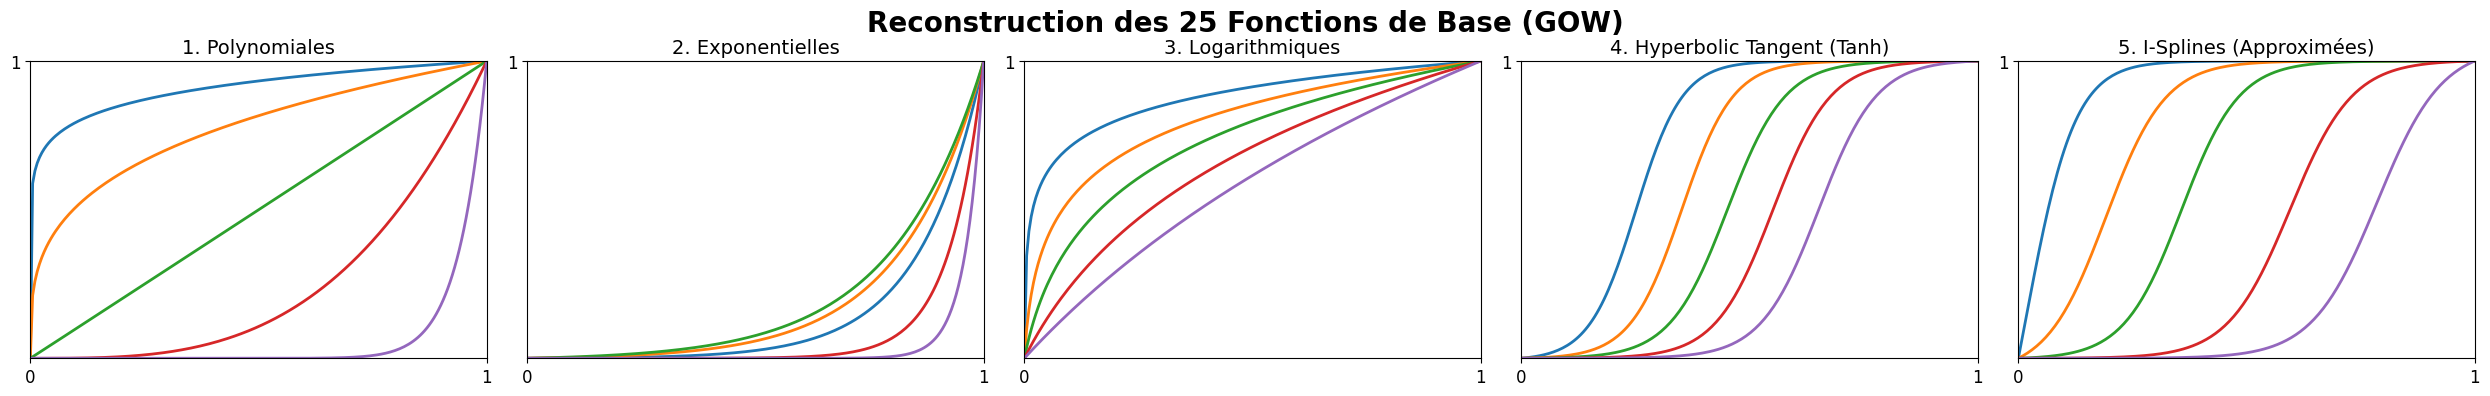
\includegraphics[width=0.92\linewidth]{25_courbes}
  \vspace{-4pt}\caption{\small Les 25 fonctions de base reconstruites par rétro-ingénierie~\cite{gow2025}.}
  \label{fig:25_courbes}
\vspace{-6pt}
\end{figure}

\textbf{Hyperparamètres.} Nous utilisons $\lambda_1 = 5$ (dans la plage de
stabilité $[1, 100]$ identifiée par~\cite{gow2025}) et $\lambda_2 = 10$
(valeur par défaut du dépôt\footnotemark[\getrefnumber{fn:repo}],
non réoptimisée).

\begin{figure}[htb]
  \vspace{-2pt}
  \centering
  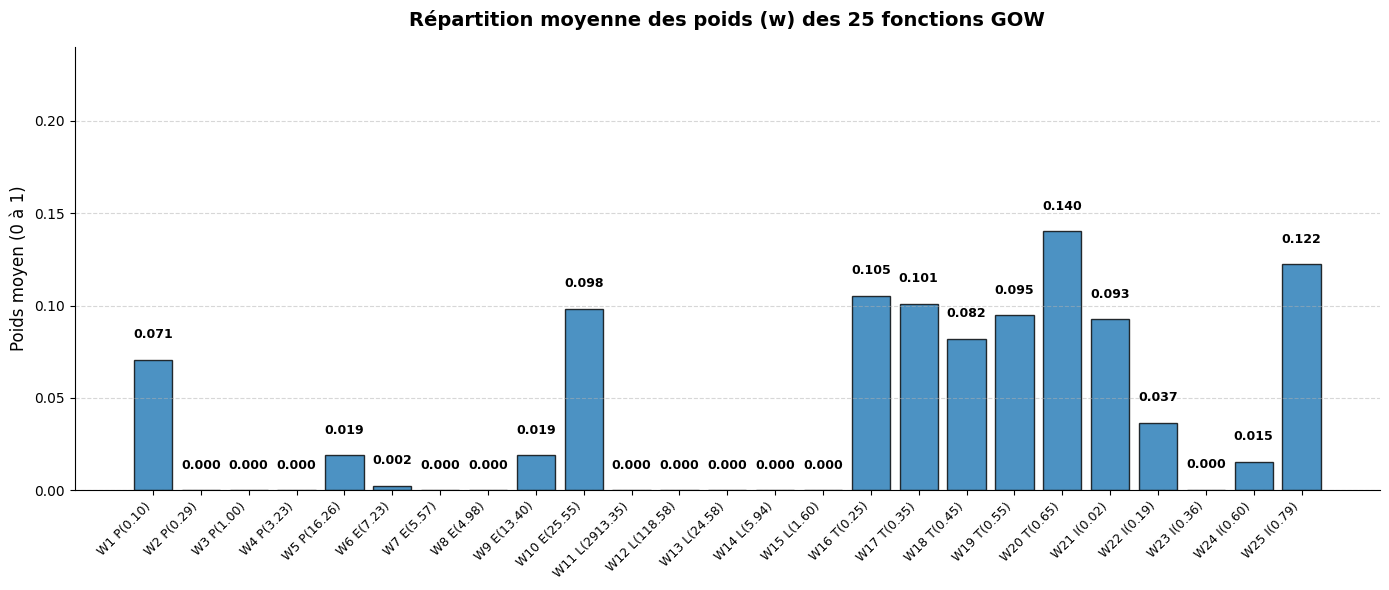
\includegraphics[width=0.98\linewidth]{poids_gow}
  \vspace{-4pt}\caption{\small Distribution des poids $w$ par essai expérimental pour GOW.}
  \label{fig:gow_weights}
\vspace{-6pt}
\end{figure}

\subsubsection{POW : Partial Ordered Wasserstein}

POW étend le transport optimal ordonné en relâchant la contrainte de
transport exhaustif : seule une fraction $s \in (0,1]$ de la masse totale
est transportée, ce qui permet d'ignorer les portions du signal les plus
coûteuses à aligner, artefacts, bruits périphériques ou silences
parasites~\cite{pow2024}. Le paramètre $\lambda$ pénalise les correspondances
éloignées de la diagonale temporelle ($\lambda(i/N - j/M)^2$), maintenant
une cohérence temporelle globale tout en autorisant des distorsions locales.

La construction de la matrice de coût est identique à GOW.

\textbf{Hyperparamètres.} $\lambda = 5$ (cohérent avec les expériences du
papier POW sur des datasets de référence). Pour $s$, le papier propose
d'estimer dynamiquement la masse optimale via la dérivée seconde de la courbe
POW($s$). Nous avons implémenté cette procédure, mais calculer un $s^*$
distinct pour (TGT, X) et (OTH, X) revient à soustraire deux distances
définies sur des proportions de signal différentes, introduisant un biais
inacceptable ; utiliser le $s^*$ d'une paire pour les deux supposerait de
connaître la vérité-terrain. Nous retenons donc $s = 0{,}95$ comme valeur
globale fixe.

% ---------------------------------------------------------------
\section{Résultats et évaluation}
\label{sec:resultats}

\subsection{Métriques d'évaluation}

\subsubsection{Filtrage du dataset}
\label{sec:filtrage}

L'analyse exploratoire a révélé deux anomalies. \textbf{Profils de certitude
hétérogènes :} certains auditeurs n'utilisent que les extrêmes ($\pm3$),
d'autres que $\pm1$, indépendamment de leur taux de réussite. Nous
appliquons une normalisation intra-participant alignant la certitude moyenne
de chacun sur la valeur médiane de l'échelle, avant restauration du signe.
\textbf{Anomalie d'overlap :} 9 paires d'auditeurs francophones et 7 paires
anglophones ont reçu des listes d'essais identiques (anomalie du générateur
aléatoire). Or, malgré des listes identiques, ces auditeurs n'ont pas produit
des scores identiques, ce qui valide que ce ne sont pas des doublons. 
Pour éviter ce biais artificiel dans l'échantillon, un membre de chaque paire a donc été exclu.

Ces deux filtrages n'affectent pas qualitativement les conclusions de l'étude,
démontrant la robustesse des modèles face au bruit d'annotation. 
La hiérarchie des performances reste strictement identique sans ces filtres. 
Sur les Odds Ratios du corpus anglophone, l'ordre GOW $>$ POW $>$ DTW est
préservé ($\text{OR} = 2{,}06$ ; $1{,}95$ ; $1{,}84$ sans filtre contre
$2{,}08$ ; $2{,}00$ ; $1{,}86$ avec filtre). De même, pour les corrélations
continues globales sur le corpus francophone, POW conserve sa supériorité
systématique ($r = 0{,}285$ pour POW $>$ $0{,}261$ pour GOW $>$ $0{,}258$
pour DTW sans filtre, contre $r = 0{,}288$ $>$ $0{,}264$ $>$ $0{,}261$ avec
filtre). L'application de ces filtres se contente donc de lisser marginalement
le bruit inter-annotateurs sans créer d'avantages artificiels pour
les modèles de Transport Optimal.

\subsubsection{Métriques retenues}
\label{sec:metriques_retenues}

Notre objectif n'est pas de concevoir un classifieur parfait, mais d'évaluer
dans quelle mesure POW et GOW simulent le comportement perceptif humain. Nous
articulons l'évaluation autour de cinq métriques.

\textbf{L'Accuracy Globale} (performance brute) vérifie la viabilité
mathématique des algorithmes et fournit un point de repère, notamment par
rapport à la performance humaine (cf.~section~\ref{sec:resultats_details}).

\textbf{Les Corrélations inter-modèles} quantifient l'apport géométrique
réel de chaque distance avant toute comparaison aux humains. Parmi les
métriques présentées ci-dessous, nous qualifions de \textit{cognitives} les
Tables de Contingence (Odds Ratio) et les Corrélations Humain-Machine par
triplet, dans la mesure où elles confrontent directement le
comportement du modèle aux réponses perceptives humaines.

\textbf{Le Plafond cognitif (Humain vs.\ Humain).} La perception de la
parole est bruitée et subjective. Nous divisons aléatoirement les
participants en deux groupes de taille égale et confrontons, essai par
essai, leurs évaluations respectives ; cette répartition aléatoire est
répétée 1\,000 fois afin d'obtenir une estimation stable (moyenne et écart-type)
de la corrélation et de l'Odds Ratio maximaux atteignables sur ce corpus,
utilisés comme référence supérieure.

\textbf{Les Tables de Contingence Humain vs.\ Modèle.} En croisant la
décision binaire du modèle et celle de l'humain essai par essai, l'Odds
Ratio~\cite{oddsratio} quantifie si les erreurs du modèle coïncident
structurellement avec celles des auditeurs humains. Le test de
McNemar~\cite{mcnemar} évalue la significativité statistique de cette
association sur table de contingence $2 \times 2$.

\textbf{La Corrélation Humain-Machine par triplet} évalue si le
delta continu du modèle évolue proportionnellement à la difficulté perçue
par les auditeurs. L'unité d'analyse est ici le triplet (moyenne
sur les essais partageant les mêmes types linguistiques, soit en moyenne
environ 3,29 essais par triplet), ce qui lisse la variabilité
individuelle.

\subsection{Résultats}
\label{sec:resultats_details}

\subsubsection{Fidélité du pipeline et corrélations inter-modèles}

Notre DTW présente une corrélation de Pearson $r = 0{,}999$ avec le DTW
de référence du dataset, ce qui valide la quasi-parfaite fidélité de notre
pipeline d'extraction par rapport au dépôt de référence.
La figure~\ref{fig:corr_models} présente les nuages de points des deltas
entre chaque paire de modèles.
POW et DTW ($r = 0{,}920$) : forte corrélation attendue (objectif
d'alignement temporel partagé, malgré des cadres théoriques distincts), mais la dispersion confirme que POW introduit une
géométrie distincte. GOW présente les corrélations
les plus faibles : $r = 0{,}842$ avec DTW et $r = 0{,}912$ avec POW,
confirmant que les déformations non-linéaires réorganisent substantiellement
l'espace de décision. La corrélation GOW-POW plus élevée que GOW-DTW
s'explique par leur cadre théorique commun (Transport Optimal).

\begin{figure}[htb]
  \vspace{-2pt}
  \centering
  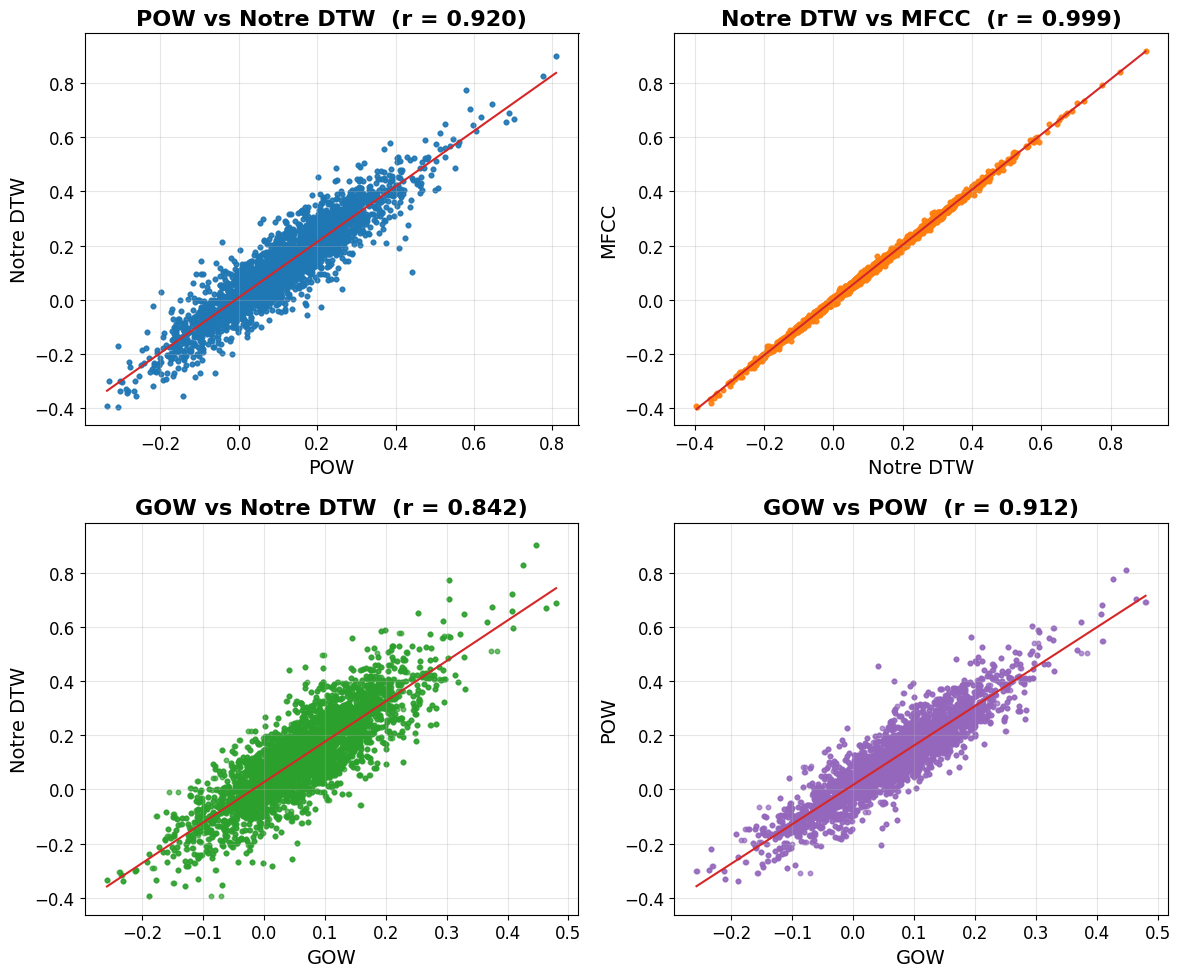
\includegraphics[width=0.78\linewidth]{corr_models}
  \vspace{-4pt}\caption{\small Nuages de points des deltas entre chaque paire de modèles
  (Notre DTW, POW, GOW, DTW de référence).}
  \label{fig:corr_models}
\vspace{-6pt}
\end{figure}

\subsubsection{Plafond humain vs. humain}

\textbf{Par essai expérimental} (référence pour les tables de contingence) :
$r = 0{,}24 \pm 0{,}008$. Les deux demi-groupes s'accordent dans 75,5\% des
cas (69,9\% de réussites communes, 5,6\% d'erreurs communes), avec 12,2--12,3\%
de désaccords. L'Odds Ratio vaut $\text{OR} = 2{,}61$ : lorsqu'un groupe se
trompe, l'autre a 2,61 fois plus de chances de se tromper également, preuve
que l'erreur est structurée par l'ambiguïté acoustique. Cet OR constitue le
plafond de référence.

\textbf{Par triplet} (référence pour les corrélations) : en agrégeant
par type linguistique de stimulus (en moyenne 3,29 essais par type), la
variabilité individuelle se lisse et la corrélation monte à
$r = 0{,}41 \pm 0{,}013$, soit la limite supérieure atteignable sur ce corpus.

\subsubsection{Tables de contingence}

La figure~\ref{fig:contingence} présente les tables de contingence humain
vs.\ modèle pour chaque langue.

\textbf{Accuracy brute.} Les humains atteignent 79,5\% en
anglais et 84,1\% en français. Les modèles sont comparables
entre eux : en anglais, DTW 78,9\%, POW 78,1\%, GOW 75,4\% ; en français,
DTW 78,1\%, POW 79,6\%, GOW 76,7\%.

\textbf{Structure de l'erreur, corpus anglophone.} DTW ($\text{OR} = 1{,}86$,
$p = 0{,}364$) : les désaccords avec les humains ne sont pas statistiquement
structurés. POW ($\text{OR} = 2{,}00$, $p < 0{,}05$) et GOW
($\text{OR} = 2{,}08$, $p < 0{,}001$) améliorent significativement ce
résultat, GOW atteignant $\approx 80$\% du plafond humain (2,61).

\textbf{Structure de l'erreur, corpus francophone.} La hiérarchie est
identique, avec une significativité très forte pour tous les modèles : DTW
($\text{OR} = 1{,}72$, $p < 0{,}001$), POW ($\text{OR} = 1{,}97$,
$p < 0{,}001$), GOW ($\text{OR} = 1{,}94$, $p < 0{,}001$). Les OR
inférieurs à ceux de l'anglais s'expliquent par la plus grande diversité
des contrastes français (249 contre 212), rendant la tâche structurellement
plus variable.

DTW, contraint par son alignement exhaustif, capture la structure de
l'erreur humaine de façon non significative en anglais. POW et GOW, en
relâchant ces contraintes, la reproduisent significativement mieux dans
les deux langues.

\begin{figure}[htb]
  \vspace{-2pt}
  \centering
  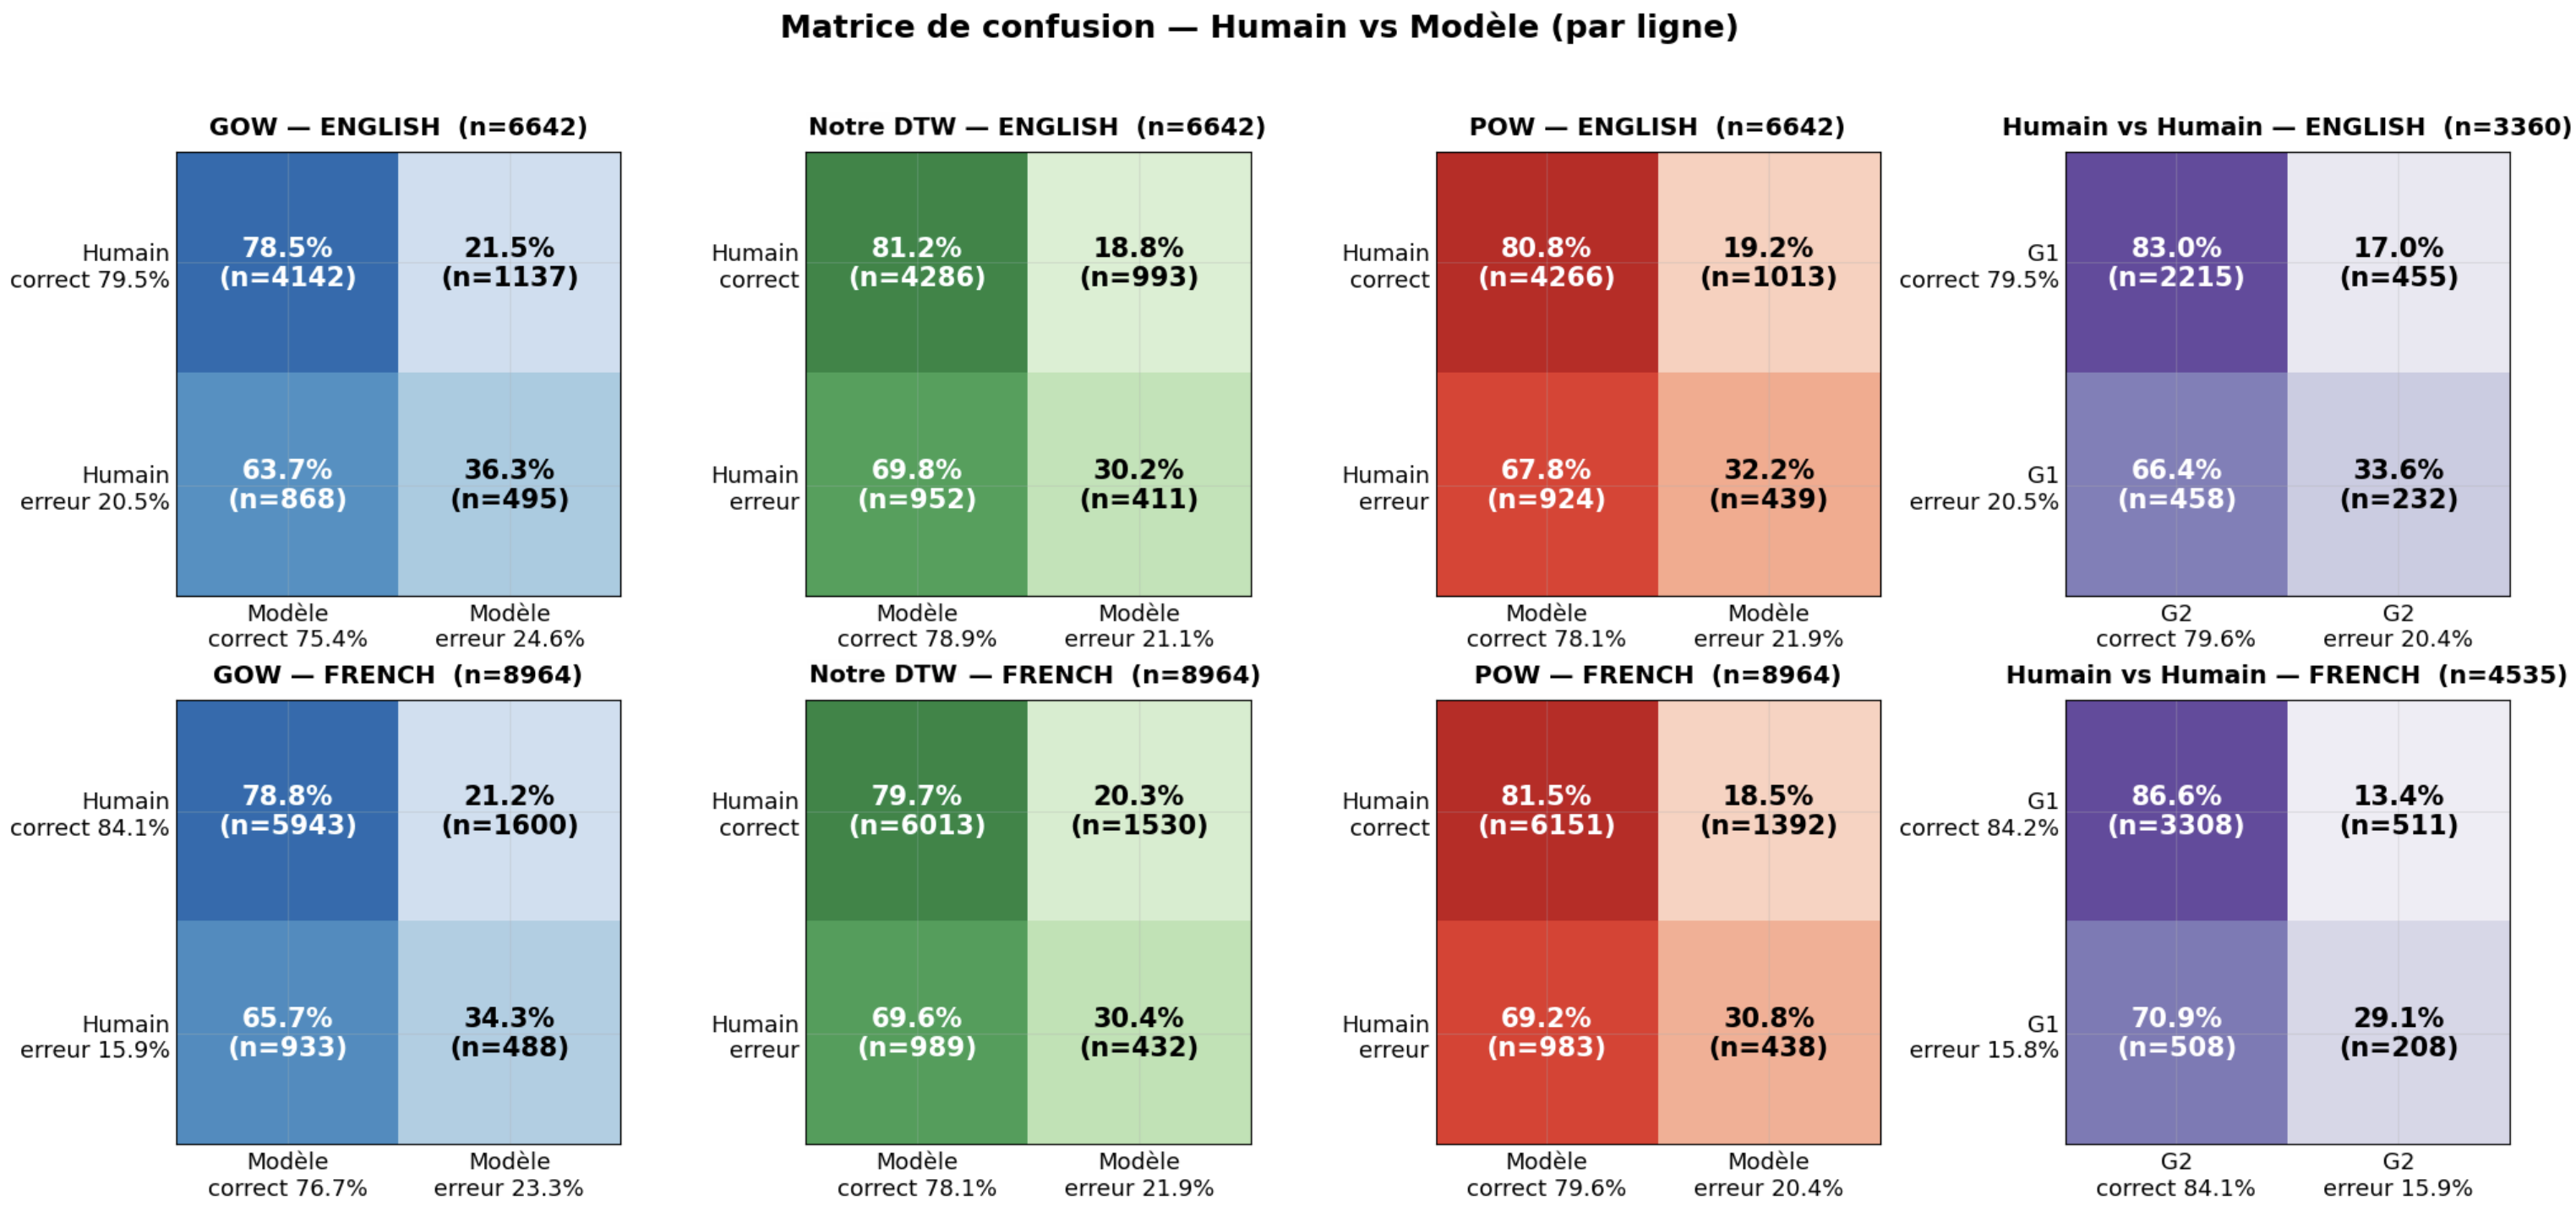
\includegraphics[width=0.78\linewidth]{contingence}
  \vspace{-4pt}\caption{\small Tables de contingence humain vs.\ modèle par langue
  (Notre DTW, POW, GOW et plafond humain vs.\ humain).}
  \label{fig:contingence}
\vspace{-6pt}
\end{figure}

\subsubsection{Corrélations humain-machine par triplet}

Plafond de référence : $r = 0{,}41 \pm 0{,}013$.

\textbf{Corrélation modèle-humain (Figure~\ref{fig:corr_global}).} Toutes les
corrélations sont hautement significatives ($p < 10^{-23}$). En français :
POW $r = 0{,}288$, GOW $r = 0{,}264$, DTW $r = 0{,}261$. En anglais : POW
$r = 0{,}333$, GOW $r = 0{,}314$, DTW $r = 0{,}292$ (64 à 81\% du plafond).

\begin{figure}[htb]
  \vspace{-2pt}
  \centering
  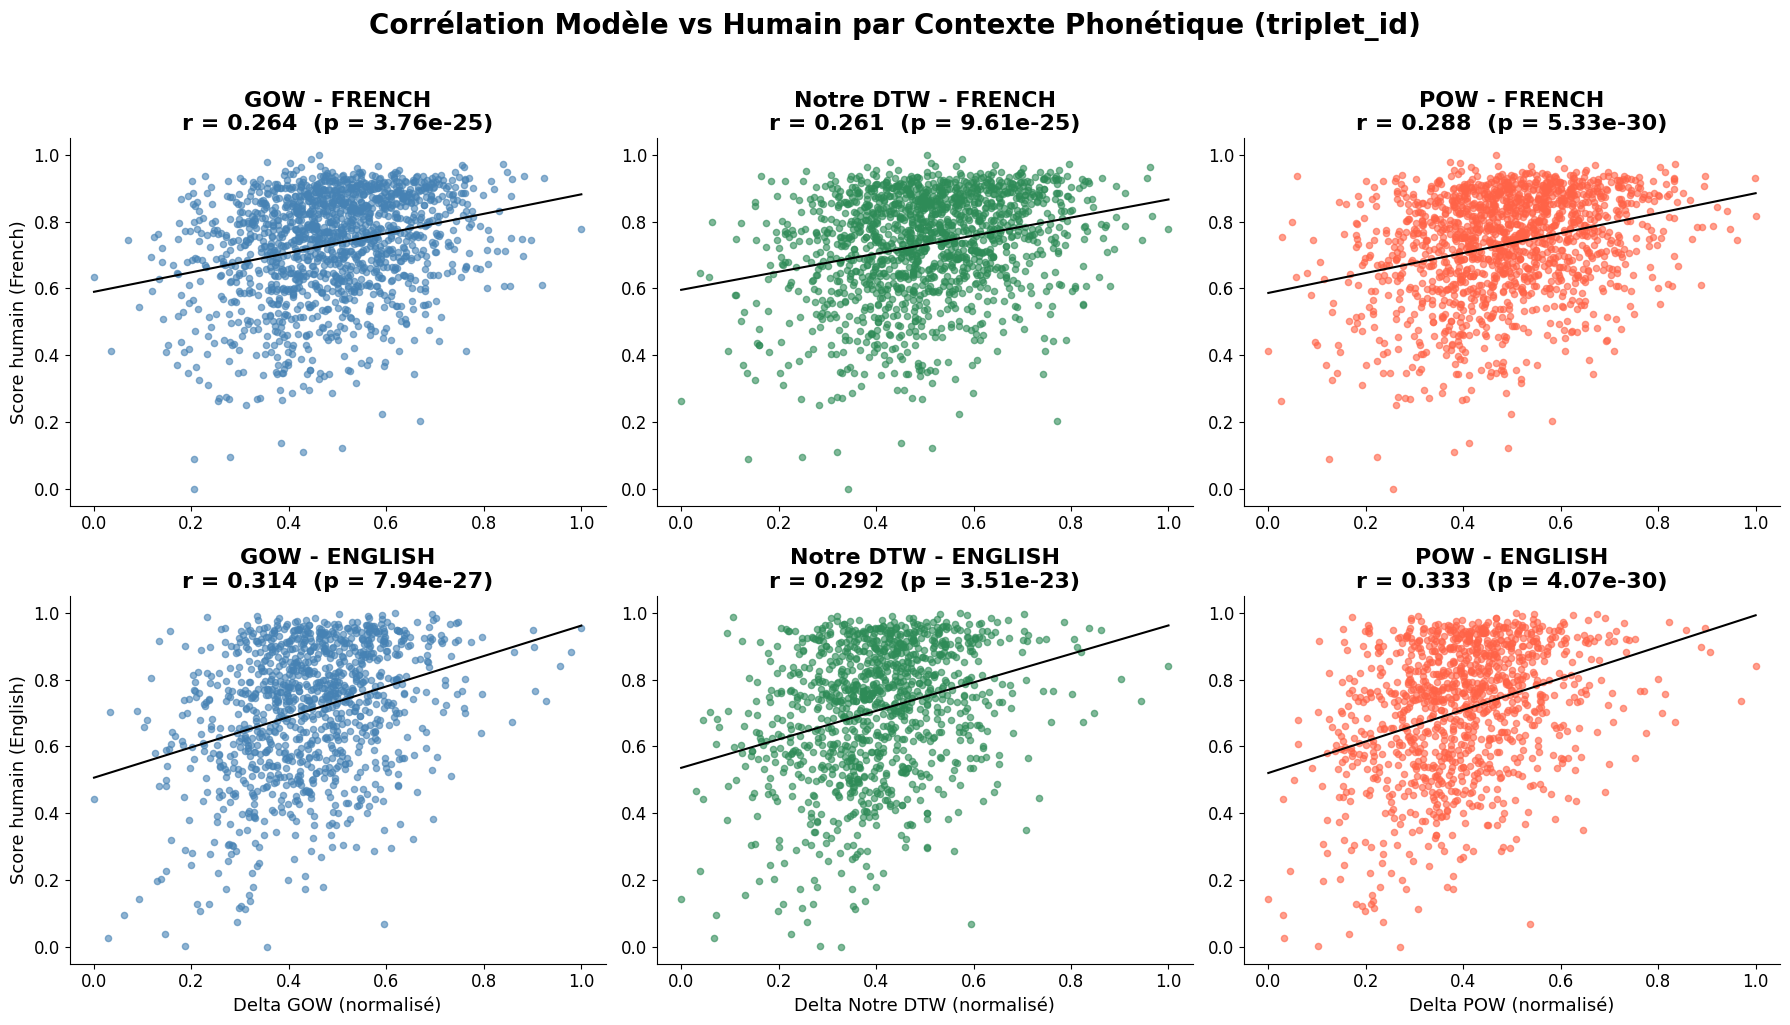
\includegraphics[width=0.78\linewidth]{corr_humain_comp}
  \vspace{-4pt}\caption{\small Corrélation modèle-humain par triplet (contexte phonétique global).}
  \label{fig:corr_global}
\vspace{-6pt}
\end{figure}

\textbf{Types de triplets réussis par les humains (Figure~\ref{fig:corr_reussite}).}
Les corrélations baissent mais restent significatives. En français : DTW
$r = 0{,}230$, POW $r = 0{,}225$, GOW $r = 0{,}219$. En anglais : POW
$r = 0{,}213$, GOW $r = 0{,}211$, DTW $r = 0{,}183$.

\begin{figure}[htb]
  \vspace{-2pt}
  \centering
  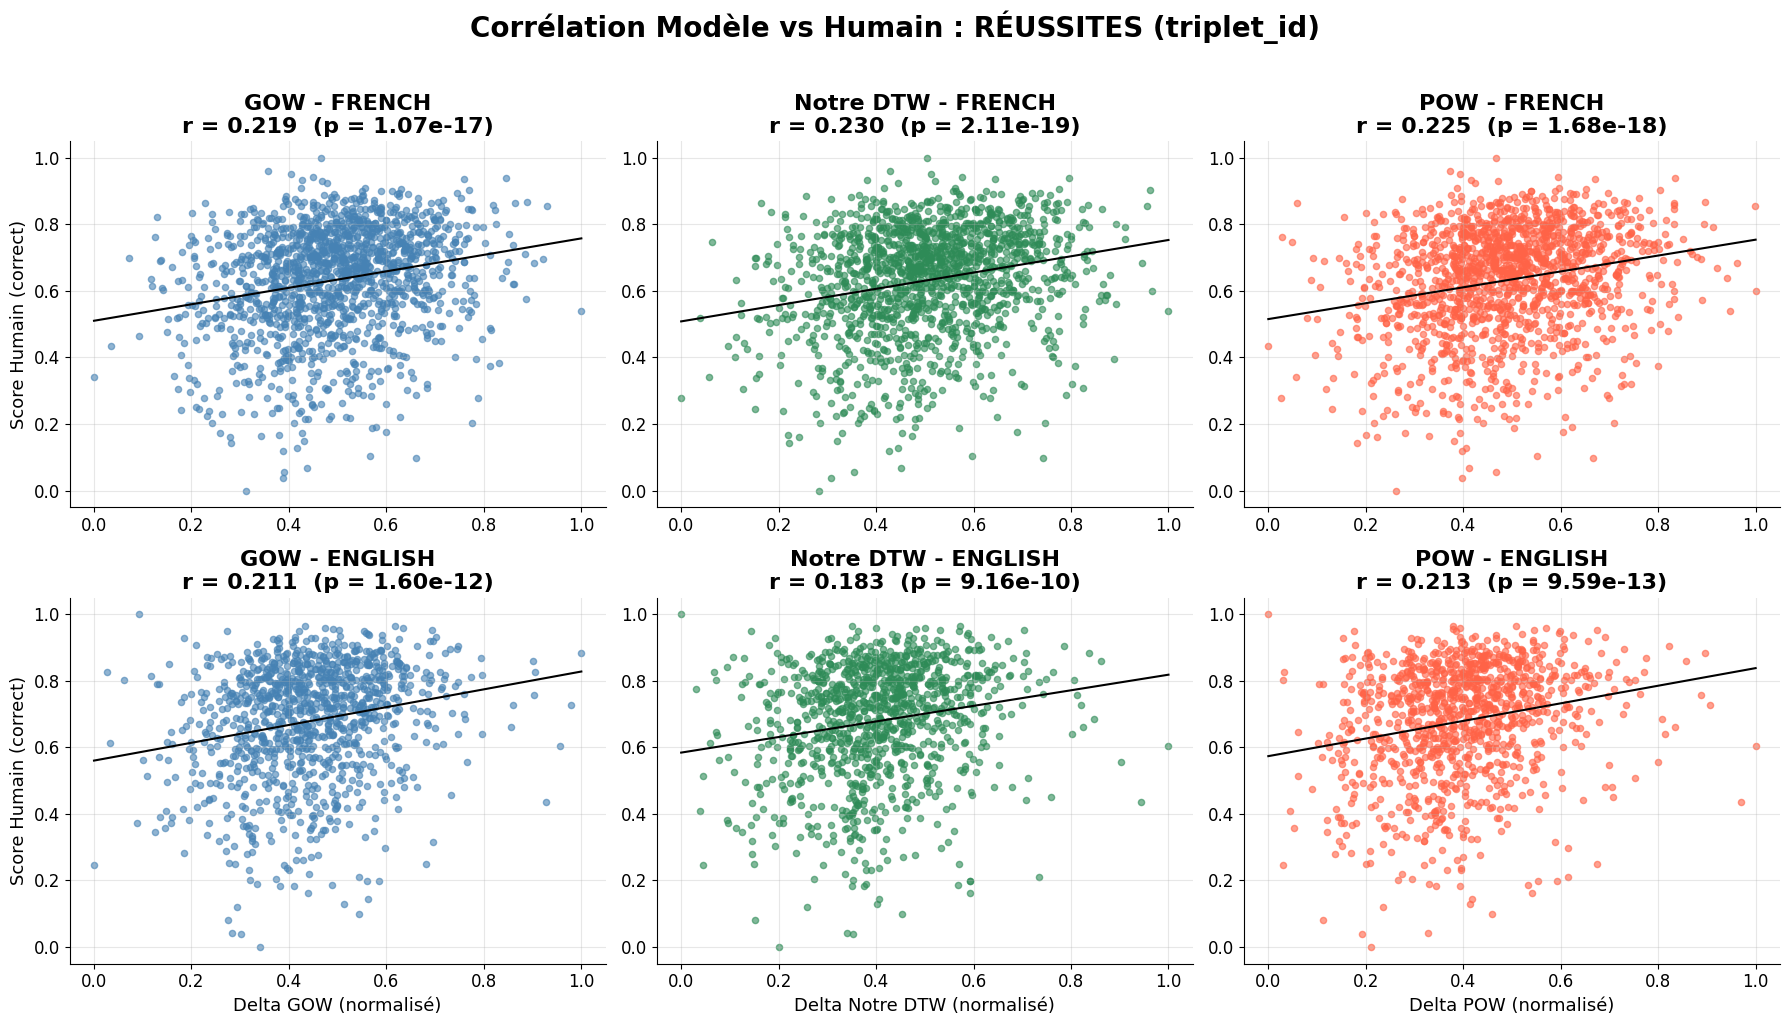
\includegraphics[width=0.78\linewidth]{corr_humain_reussite}
  \vspace{-4pt}\caption{\small Corrélation modèle-humain sur les types de triplets réussis par les humains.}
  \label{fig:corr_reussite}
\vspace{-6pt}
\end{figure}

\textbf{Types de triplets ratés par les humains (Figure~\ref{fig:corr_erreur}).}
Les corrélations s'effondrent et deviennent non significatives en français
(GOW $r = -0{,}019$, $p = 0{,}615$ ; DTW $r = 0{,}005$, $p = 0{,}889$ ;
POW $r = 0{,}021$, $p = 0{,}549$), et en anglais ($r \approx 0{,}07$).
Sur ces zones d'ambiguïté, aucun modèle ne dispose de signal
acoustique suffisant pour ordonner la difficulté : le delta fluctue
aléatoirement, comme un auditeur face à un contraste indiscernable.

\begin{figure}[htb]
  \vspace{-2pt}
  \centering
  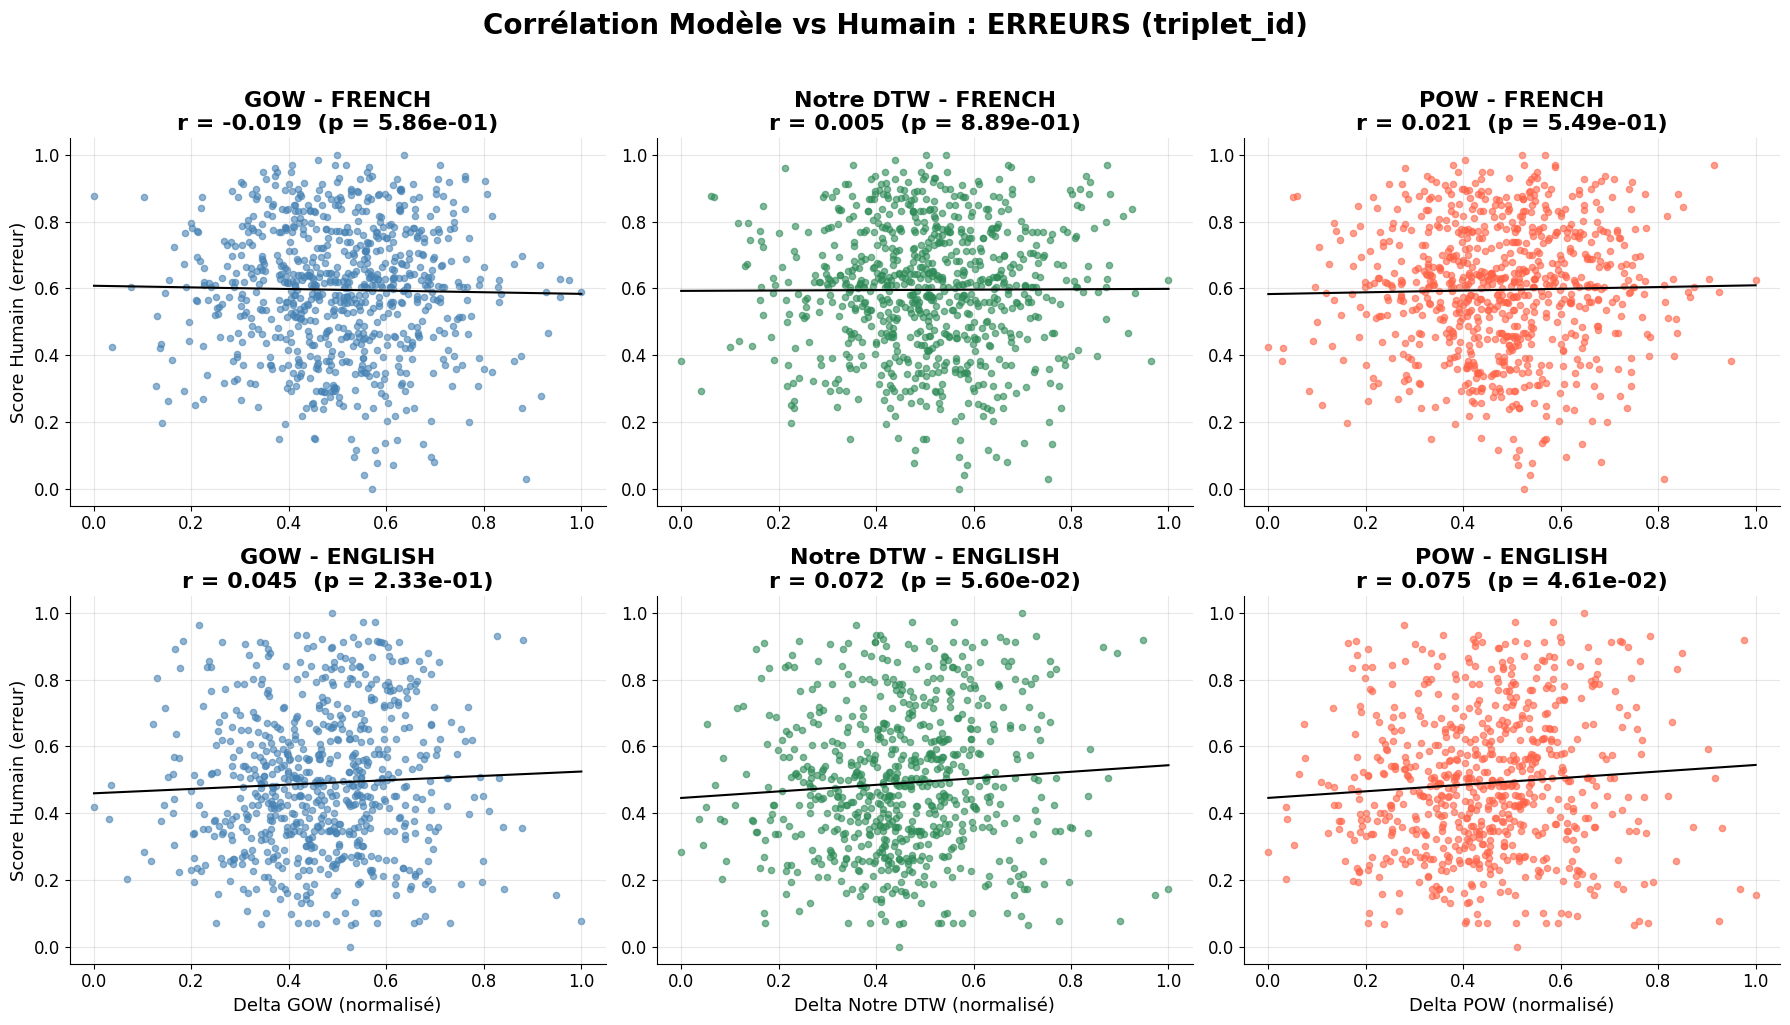
\includegraphics[width=0.78\linewidth]{corr_humain_err}
  \vspace{-4pt}\caption{\small Corrélation modèle-humain sur les types de triplets ratés par les humains.}
  \label{fig:corr_erreur}
\vspace{-6pt}
\end{figure}

La corrélation continue est portée presque exclusivement par les contrastes
que les humains réussissent. POW présente l'avantage le plus consistant dans
les deux langues pour cette métrique, suggérant que le filtrage des outliers
acoustiques aligne mieux la certitude du modèle sur la difficulté perçue.

% ---------------------------------------------------------------
\section{Discussion et perspectives}
\label{sec:discussion}

\subsection{Synthèse}

Sur l'accuracy brute (75--80\%), les trois modèles sont comparables, validant
la viabilité des implémentations. Les différences s'affirment sur les
métriques cognitives : les tables de contingence montrent que DTW reproduit
la structure de l'erreur humaine de façon non significative en anglais,
tandis que POW et GOW l'améliorent significativement (OR jusqu'à 2,08, soit
80\% du plafond de 2,61). Les corrélations continues par triplet
confirment cet avantage, POW présentant les meilleures valeurs dans les deux
langues ($r = 0{,}288$ en français, $r = 0{,}333$ en anglais).

Ces deux métriques sondent des aspects complémentaires de l'accord
humain-machine. Les tables de contingence évaluent si le modèle commet
les mêmes erreurs discrètes que les humains essai par essai (GOW légèrement
meilleur en anglais, OR 2,08 vs 2,00). La corrélation continue mesure si
le delta du modèle reflète la certitude gradée des auditeurs au niveau des
types de triplets (POW systématiquement meilleur). Cette dissociation est
cohérente avec la nature de POW : en filtrant les portions les moins fiables
du signal ($s = 0{,}95$), POW produit des deltas plus proches du niveau de
performance brute humain, ce qui se traduit par une meilleure prédiction de
la difficulté graduée. GOW, dont la déformation non-linéaire apprend à
distinguer les contrastes difficiles des faciles, capture mieux la
binarisation de l'erreur. Les deux approches sont donc complémentaires
plutôt que concurrentes.

\subsection{Limites}

Les corrélations, bien que hautement significatives, demeurent modestes
($r \approx 0{,}26$--$0{,}33$). Cet écart par rapport au plafond
($r = 0{,}41$) reflète en partie les différences interindividuelles entre
participants, le plafond humain vs.\ humain intègre déjà cette variabilité
et représente donc la limite atteignable sur ce corpus, non une cible
absolue. Une autre part de l'écart découle de la représentation MFCC,
modélisation de bas niveau surpassée par les représentations latentes
profondes multilingues~\cite{perceptimatic2020}.

Par ailleurs, les stimuli sont courts (237\,ms en moyenne) et ont été
manuellement nettoyés et réalignés~\cite{perceptimatic2020}, minimisant
précisément les artefacts que GOW et POW sont théoriquement conçus pour
gérer. Leurs avantages sont donc structurellement sous-exploités dans ce
corpus.

\subsection{Perspectives}

La direction prioritaire est la substitution des MFCC par des embeddings
issus de modèles profonds multilingues (type S2 de Perceptimatic), afin de
déterminer si POW et GOW apportent un gain similaire sur des représentations
de plus haut niveau, et notamment si l'on peut saturer le plafond perceptif
référence humaine. Il serait également pertinent de les évaluer sur des
séquences plus longues et non pré-segmentées, où les distorsions temporelles
et outliers acoustiques sont réellement présents.

% ---------------------------------------------------------------
\clearpage
\section*{Références}
\label{sec:refs}
\begin{thebibliography}{99}
\small
\setlength{\itemsep}{0pt}
\setlength{\parskip}{0pt}

\bibitem{pow2024}
T.~Doan, T.~Phan, P.~Nguyen, K.~Than, M.~Visani, A.~Takasu,
\enquote{Partial Ordered Wasserstein Distance for Sequential Data,}
\textit{Neurocomputing}, 2024.

\bibitem{gow2025}
T.~Doan, H.~To, H.~Vuong, M.~Visani, A.~Takasu, K.~Than,
\enquote{Generalized Ordered Wasserstein Distance,}
\textit{Pattern Recognition}, 2025.

\bibitem{perceptimatic2020}
J.~Millet, E.~Dunbar,
\enquote{Perceptimatic: A Human Speech Perception Benchmark for Unsupervised
Subword Modelling,}
\textit{Proc. Interspeech}, 2020.

\bibitem{zerospeech2017}
E.~Dunbar, X.~N.~Cao, J.~Benjumea, J.~Karadayi, M.~Bernard,
L.~Besacier, X.~Anguera, E.~Dupoux,
\enquote{The Zero Resource Speech Challenge 2017,}
in \textit{Proc. IEEE Workshop on Automatic Speech Recognition and
Understanding (ASRU)}, IEEE, 2017, pp.~323--330.

\bibitem{mfcc}
S.~B.~Davis, P.~Mermelstein,
\enquote{Comparison of Parametric Representations for Monosyllabic Word
Recognition in Continuously Spoken Sentences,}
\textit{IEEE Trans. Acoust. Speech Signal Process.}, vol.~28, no.~4,
pp.~357--366, 1980.

\bibitem{dtw}
H.~Sakoe, S.~Chiba,
\enquote{Dynamic Programming Algorithm Optimization for Spoken Word
Recognition,}
\textit{IEEE Trans. Acoust. Speech Signal Process.}, vol.~26, no.~1,
pp.~43--49, 1978.

\bibitem{Drop-DTW}
N.~Dvornik, I.~Hadji, K.~G.~Derpanis, A.~Garg, A.~D.~Jepson,
\enquote{Drop-DTW: Aligning Common Signal Between Sequences While Dropping
Outliers,}
in \textit{Advances in Neural Information Processing Systems (NeurIPS)},
2021.

\bibitem{optimal_transport}
C.~Villani,
\textit{Topics in Optimal Transportation},
Graduate Studies in Mathematics, vol.~58,
American Mathematical Society, Providence, RI, 2003.

\bibitem{phoneme}
International Phonetic Association,
\textit{Handbook of the International Phonetic Association:
A Guide to the Use of the International Phonetic Alphabet},
Cambridge University Press, Cambridge, 1999.

\bibitem{github_perceptimatic}
J.~Millet, E.~Dunbar,
\enquote{Perceptimatic -- Source code repository,}
GitHub, 2020.
\url{https://github.com/JAMJU/interspeech-2020-perceptimatic}

\bibitem{kaldi}
D.~Povey, A.~Ghoshal, G.~Boulianne, L.~Burget, O.~Glembek, N.~Goel,
M.~Hannemann, P.~Motlicek, Y.~Qian, P.~Schwarz, J.~Silovsky,
G.~Stemmer, K.~Vesely,
\enquote{The Kaldi Speech Recognition Toolkit,}
in \textit{Proc. IEEE Workshop on Automatic Speech Recognition and
Understanding (ASRU)}, IEEE Signal Processing Society, 2011.

\bibitem{plotdigitizer}
Plot Digitizer.
\url{https://plotdigitizer.com}

\bibitem{github_project}
\url{https://github.com/RL-I3A/pow-gow-perceptimatic-2026.git}

\bibitem{github_gow}
H.~To, T.~Doan,
\enquote{Generalized Ordered Wasserstein -- Source code repository,}
GitHub, 2025.
\url{https://github.com/TungDP/GOW}

\bibitem{github_pow}
T.~Doan,
\enquote{Partial Ordered Wasserstein Distance -- Source code repository,}
GitHub, 2024.
\url{https://github.com/TungDP/Partial-Ordered-Wasserstein-Distance}

\bibitem{oddsratio}
J.~M.~Bland, D.~G.~Altman,
\enquote{Statistics Notes: The Odds Ratio,}
\textit{BMJ}, vol.~320, no.~7247, p.~1468, 2000.

\bibitem{mcnemar}
Q.~McNemar,
\enquote{Note on the Sampling Error of the Difference between Correlated
Proportions or Percentages,}
\textit{Psychometrika}, vol.~12, no.~2, pp.~153--157, 1947.
\url{https://doi.org/10.1007/BF02295996}

\end{thebibliography}

\end{document}